%This work is licensed under the Creative Commons Attribution-ShareAlike 4.0
%International License. To view a copy of this license, visit
%http://creativecommons.org/licenses/by-sa/4.0/.
%
\documentclass[a4paper]{IEEEtran}
\usepackage[utf8]{inputenc}
\usepackage[T1]{fontenc}
\usepackage{microtype}
\usepackage{amsmath}
\usepackage{amssymb}
\usepackage{amsfonts}
\usepackage[pdftex]{graphicx}
\usepackage{color}
\usepackage{xspace}
\usepackage{array}
\newcommand{\gr}{GNU\,Radio\xspace}
\newcommand{\grc}{\texttt{grc}\xspace}
\newcommand{\gsoc}{Google\,Summer\,of\,Code\xspace}
\newcommand{\grbench}{\texttt{gr-benchmark}\xspace}
\newcommand{\zeromq}{\texttt{$\varnothing$MQ}\xspace}
\author{Marcus Müller,~BSc. \\[1.2em]%
{\scriptsize \texttt{marcus@hostalia.de}\\%
\texttt{funkylab} on freenode.org}\\[1.2em]%
%
{\footnotesize Karlsruhe, Germany\\Student at the Karlsruhe Institute of Technology}}
\title{Performance Measurement Toolbox for \gr}
\usepackage[final=true]{hyperref}
\hypersetup{
	pdfauthor = {Marcus Müller},
	pdftitle = {Google Summer of Code 2014 proposal: Performance Measurement Toolbox for \gr},
	pdfsubject = {Performance Measurement Toolbox for \gr},
%	hidelinks = {true}
}
\IEEEspecialpapernotice{\gsoc 2014}
\begin{document}
\maketitle

\begin{abstract} \gr has become one of the most popular frameworks for
development of experimental wireless transceiver systems, especially in the
research community. Research and Development however are in need of extensive
metrics of such systems. A very common task, therefore, is variation of \gr
flow graph parameters and collecting values determined by running the system,
including transceiver characteristics like bit error rate benchmarking, but
there is rising need in the digital signal processing community to gather
software performance data.

This document proproses a \gsoc project to create a unified, distributed and
versatile tool to do benchmarking of signal processing applications as a whole
and for performance analysis of their components.  \end{abstract}

\section{Background} \gr has been part of numerous research projects on
wireless transmission systems, including development of modulation schemes,
medium access control strategies and is in the process of getting a
increasingly comprehensive channel coding framework.

With the creation of \grbench, steps were taken to profile the execution of \gr
applications as well as components on different computing platforms. However,
this is limited to benchmarks run on the local computer and to extracting key
data for analysis and potential upload to a central server\cite{grbenchmark}.

For the development of complex transceiver systems, this covers but an aspect
of the overall desirable benchmarking tools:

One typical benchmark is the performance of such a system is the bit error rate
(BER) curve over varying SNR conditions. While there are plenty options to
gather data from \gr flow graphs and generate such statistics from them, there
is a distinct lack of tools that enables researchers and developers to run
extensive benchmarks in an easy, reproducible, and comfortably analyzable ways. 

Furthermore, benchmarking a complex simulation can take quite some computation
time. It is highly desirable that benchmarks can be automatically distributed
to remote systems, the results being gathered on a central node. This has to be
done by a system that \emph{guarantees} that results are properly labeled,
archived, the parameters documented and stored in a way that enables
visualization as much as sharing and analysis using standard tools.

The main objective of \grbench is to profile the computational performance of
different implementation of algorithms and mathematical base operation,
especially for the VOLK library\cite{volk}; it implements a method to upload
profiling data to the central \url{http://stats.gnuradio.org} server for
analysis by the VOLK community.  Obviously, it is desirable that when
developing performance-critical code one is able to test performance on several
machines while coding is still in progress, and not just when code is
\textit{out in the wild}; that's basically the same reason \gr encourages
developers to use the tightly integrated unit testing tools when developing in
and out of tree modules.

This brings up the need for a centralized dispatcher mechanism that distributes
the execution of benchmarks to different machines according to rules that
either govern the execution of each benchmark on each machine for computational
profiling and testing purposes or the minimization of the execution time of a
benchmark suite for processing performance benchmarking.

\section{Proposed Project}

\subsection{Extension of \grbench}

\subsubsection*{Application performance measurement} So far, \grbench is
tailored to the need of the VOLK community to benchmark specific
implementations of mathematical routines on different architectures.

This leaves room for unforeseen behaviour: Running a highly optimized VOLK
kernel in a benchmark potentially provides the kernel with CPU cores for nearly
exclusive use; realistically, these kernels are part of larger \gr
applications.  This leads to competition for CPU cores, and even more
importantly, for caches.  If a kernel works well on its own, it might actually
profit greatly from caching mechanisms. If, however, the complete system is
to process a larger number of sample buffers, cache misses will occur far more
often. To measure the performance of kernels, it therefore seems reasonable to
compare the time spent on the kernel with the total computation time of an
application employing that respective kernel.

\subsubsection*{Signal Processing Focus} As a very common task is the simulation
of a transceiver system under different environments (SNR, Frequency Offset,
Interference, Timing misbehavior). \grbench should be
expanded to accommodate the FEC API as well as to be configured to run
simulations with a specified set of simulation parameters. 

I anticipate that \gr users will want to have an fail-safe, easy way to get the
desired data out of the flow graph.  A set of sinks to let users specify the
data to be collected will be created; this, aside from the obvious BER, should also
include estimators for SNR, residual synchronization errors, etc.

\subsection{Dispatcher Infrastructure}

An infrastructure to remotely execute benchmarks, especially flow graphs, must
be supplied to fulfill the need for reproducible, centralized collected
distributed benchmarks.

Technologically, existing methods for the coordination should be employed.  As
a means to distribute the benchmark programs, to ensure compatible \gr versions
on all machines and to start the remote benchmarking agents, \texttt{ssh}
offers a well-established framework.

To queue individual benchmarks on the remote machines, a remote procedure call
(RPC) library should be used. Although \texttt{gr-controlport} already employs
\texttt{ICE} for RPC, which itself is networkable, defining interfaces in shape
of slices implies a considerable development overhead for the integration of
quickly changing benchmarks.

\zeromq\cite{zeromq} on the other hand has been successfully employed in GNU
Radio applications\cite{airmodes}, and already offers the optimal architecture
in an easy-to-use framework (fig.~\ref{fig:pushpull}).

\begin{figure}[h] \centering 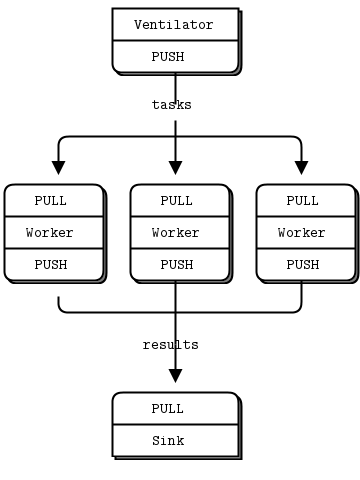
\includegraphics[width=2.4in]{pushpull.png}
\caption{\label{fig:pushpull}\zeromq-based push/pull based workload
distribution. From:
\url{http://zguide.zeromq.org/page:all\#Divide-and-Conquer}} \end{figure}

Since there are several attractive alternatives to \zeromq, such as the more
python-centered and deployment focused \texttt{execnet}\cite{execnet}, choosing
the right framework is not inherently trivial, and the decision should be one
of the initial tasks during framework development.

The dispatcher architecture must be somewhat failure tolerant: Benchmarking
results should be stored locally on the nodes, so that in case of
infrastructure failure (network outage, dispatcher crash, \dots) results are
not lost but can be collected later.

\subsubsection*{Execution of Benchmarking Plans and Storage of Results}

The overall benchmark, specifying the flow graphs, kernels or generally programs 
to be run, should be stored in \emph{plans}. The dispatcher should be able to load them
from permanent storage.

Results of Benchmarks should be stored in a relational database. For smaller plans,
an embedded database like \texttt{Sqlite3} is sufficient. Using one of the numerous
\texttt{python} RDBMS abstraction interfaces, seamless integration into high-performance
database systems should be possible.

\subsubsection*{Signal Processing Benchmark}

For computationally intensive benchmarks, distribution of benchmarking subtasks
across multiple systems is always desirable. In a lab environment, often a
rather heterogeneous network of computers is available to execute the benchmark
(fig.~\ref{fig:minimizetime}).

\begin{figure}[h] \small\centering \input{minimizetime.pdf_tex}
\caption{\label{fig:minimizetime}Benchmark distribution to achieve minimal
computation time} \end{figure}

A dispatcher user interface should enable users to run their benchmarks on the
different machines, and enable them to gather results without explicitely
assigning benchmark to the different nodes.

In this scenario, the \emph{pool manager} should have means to check the state
and availability of assigned \emph{nodes}, remove them from or add them to the
pool, monitor the individual node performance and allocate workload accordingly
to minimize total computation time.

\subsubsection*{Computational Performance Benchmark} To test e.g. optimized
algorithm on different machine types, or to gather statistical properties
(average, median, variance) of performance, benchmarks must be run on a number
of different machines simultaneously (fig.~\ref{fig:runonall}).

\begin{figure}[h] \small\centering \input{runonall.pdf_tex}
\caption{\label{fig:runonall}Benchmark distribution to all nodes, to run every
benchmark on every platform} \end{figure}

\subsection{Benchmark Design Suite}

The previous sections have shown that, depending on the benchmark type, demands
for benchmark scheduling are completely different. To account for the complexity
involved, an easy-to-use graphical interface for the planning of benchmark should
be devised.

\subsubsection*{Integration into \texttt{gnuradio-companion}}

The \grc offers users the possibility to define various variables that
can be used to parameterize blocks.

I plan \emph{Benchmark} as a new \textit{generate option} for \grc.
This will enable the user to specify \textsl{start}, \textsl{stop}, and a number of
\textsl{steps} of each parameter in a dedicated input window listing all user-specified
variables, as well as the desired number of \textsl{repetitions} per run.
These settings along with the flow graph should be exported to a \emph{plan} that can be
dispatched. Since graphical sinks do not make much sense in remotely executed benchmarks,
integration of the GUI toolkit environments into that generate option is currently not 
planned.

The generated benchmarks should be exported in dispatcher-loadable plans. 

\begin{figure}[h]
\centering
\fbox{\parbox{0.95\columnwidth}{\centering%
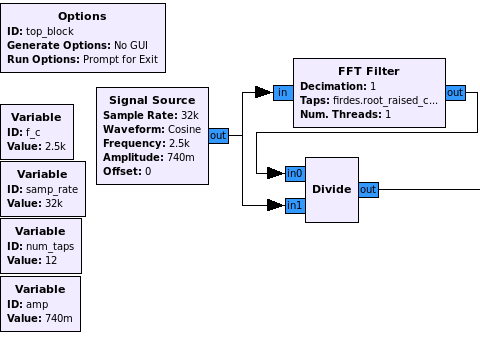
\includegraphics[width=2.4in]{grc.png}\\%
Flow Graph Design in \grc}}

$\downarrow$

\fbox{\parbox{0.95\columnwidth}{\centering%
\begin{tabular}{|r|l|l|l|c|}\hline
\textbf{variable} & \textbf{start} & \textbf{stop} & \textbf{steps} & \textbf{dim}\\\hline
f\_c & 1e3 & 10e3 & 20 & lin\\\hline
num\_taps & 4 & 1000 & 500 & lin\\\hline
amp & 1e-5 & 1 & 100 & log\\\hline
\end{tabular}\\[1em]
Benchmark Parameterizing
}}

$\downarrow$


\fbox{\parbox{0.95\columnwidth}{\centering%
\fbox{\parbox{0.85\columnwidth}{\centering%
Loading into dispatcher}}


\begin{tabular}{ccccc}
$\downarrow$&$\downarrow$&$\downarrow$&&$\downarrow$\\
\fbox{Node 1}&\fbox{Node 2}&\fbox{Node 3}&\dots&\fbox{Node N}\\
$\downarrow$&$\downarrow$&$\downarrow$&&$\downarrow$
\end{tabular}
\fbox{\parbox{0.85\columnwidth}{\centering%
Central Result Gathering}}\\[1em]

Automated Dispatching
}}

$\downarrow$

\fbox{\parbox{0.95\columnwidth}{\centering%
\begin{tabular}{ccccc}
\multicolumn{2}{c}{\fbox{\texttt{matplotlib}}} & \fbox{CSV export} & \dots & \fbox{Upload}\\
$\downarrow$ & $\downarrow$ & & & $\downarrow$\\
\fbox{\scriptsize PDF/\TeX} & \fbox{\scriptsize Display} & & &\scriptsize\fbox{stats.gnuradio}\\
\end{tabular}\\[1em]

Data Storage/Analysis
}}

\caption{\label{fig:workflow}Typical Benchmarking workflow}
\end{figure}
\subsection{Benchmark Analysis}

Publication is a necessity for scientific progress to be available to every researcher.
To ease the generation of visuals from the gathered benchmark data, the toolbox will come 
with scripts that analyze the stored benchmarking results, extract the desired data, and 
export it to comma-separated-value files, plot it directly using \texttt{matplotlib} ready
for \LaTeX{} import, or publish it (in the case of performance data) to an online statistic website.

\section{Deliverables}
\subsection{Extension of \grbench}
\begin{itemize}
\item Integration of signal processing performance Measurements
\item \grbench-enabled blocks to help users specify the relevant data
\item relative runtime measurements under load
\item Focus on statistical properties (average, variance etc.)
\end{itemize}
\subsection{Dispatcher Infrastructure}
\begin{itemize}
\item \texttt{SSH} infrastructure
	\begin{itemize}
	\item automatic login via public key authentication
	\item pool management
	\item starting of execution agents
	\end{itemize}
\item Pool manager
	\begin{itemize}
	\item add, remove nodes
	\item start agents from CLI
	\end{itemize}
\item Execution agents
	\begin{itemize}
	\item RPC infrastructure
	\item local data storage
	\item transmission format (XML?)
	\end{itemize}
\item Dispatcher
	\begin{itemize}
	\item plan loading
	\item task distribution
	\item result gathering
	\item result storage (database interface)
	\item fault analysis
	\item GUI
	\end{itemize}
\item Benchmark Design Suite
	\begin{itemize}
	\item \grc integration
	\item parameter definition
	\item plan Saving
	\end{itemize}
\item Benchmark Analysis
	\begin{itemize}
	\item data extraction
	\item export facilities (CSV, \texttt{matplotlib})
	\item upload (to \url{http://stats.gnuradio.org})
	\end{itemize}
\end{itemize}

\newpage
\section{Schedule}

This schedule is rather detailed; I honestly expect it to change in the
coordination period.
\vfill

Currently I'm employed on a 9 hours per week basis, but the schedule should
leave me with enough flexibility to do \gsoc and that in parallel. Further
commitments can be reduced, even eliminated, to ensure reaching of weekly goals.

This schedule already includes the long weekends I intend to take.

\begin{tabular}{m{10ex}m{2.5in}}
April 22 \newline May 18&
\textbf{Coordination period:}
\begin{itemize}
\item refining a wish list for \grbench features
\item defining data formats, libraries used
\item defining test cases
\item setup of a VM for distributed tests
\item setup of github repo
\item fill github issue tracker with feature requests, use from thereon
\item exchange with experts (on \grc, \texttt{gr-controlport}, \dots)
\end{itemize}
active communication on IRC\newline
announcement and RFC on discuss-gnuradio\\\hline
May 19 & \textbf{Start of work period:}\newline
constant updates on github\newline
active communication via IRC, mailing list\\[1em]
May 19\newline May 24 &
\grbench extension I
\begin{itemize}
\item whole-application benchmarks
\item data extraction blocks
\end{itemize}\\\cline{2-2}
May 26\newline May 31&
Infrastructure I
\begin{itemize}
\item choose right RPC framework (\zeromq? \texttt{execnet}? \dots)
\item benchmark dispatcher
\item benchmark running agent
\end{itemize}\\\cline{2-2}
June 2\newline June 5&
Integration I
\begin{itemize}
\item dispatcher plan loading
\item plan generation GUI
\item \grc generate option
\end{itemize}\\\cline{2-2}
June 10\newline June 14 & 
Infrastructure II
\begin{itemize}
\item wrapping tasks \& results (XML?)
\item result gathering
\item result storage
\end{itemize}\\\cline{2-2}
June 17\newline June 21 &
Infrastructure III
\begin{itemize}
\item \texttt{SSH} infrastructure
	\begin{itemize}
	\item public key storage
	\item start of agent
	\item checking of \gr version
	\end{itemize}
\end{itemize}\\
\hline June 23 \newline June 27& \textbf{Mid-term evaluation submission}\\\hline
\end{tabular}
\vfill

\begin{tabular}{m{10ex}m{2.5in}}
June 30\newline July 9&
Work on supplied feedback\\\cline{2-2}
July 10\newline July 12&
Integration II
\begin{itemize}
\item local setup script
	\begin{itemize}
	\item generation of system user
	\item public key generation
	\item \texttt{pybombs} recipe
	\end{itemize}
\item update of VM
\end{itemize}\\\cline{2-2}
July 14\newline July 19&
Data Analysis I
\begin{itemize}
\item database data extraction
\item visualisation of statistical properties
\item export
\end{itemize}\\\cline{2-2}
July 21\newline July 26&
\grbench extension II
\begin{itemize}
\item refine to store data directly to local
\end{itemize}
Infrastructure IV
\begin{itemize}
\item delayed \& failure tolerant gathering of results
\item upload facilities
\end{itemize}\\\cline{2-2}
July 28\newline August 2&
\textbf{Extensive testing \& Bugfixes}
\begin{itemize}
\item deployment on different platforms
\item VM deployment to amazon EC2 (micro)
\item \gr QA integration 
\end{itemize}\\\cline{2-2}
August 4\newline August 9&
Integration IV
\begin{itemize}
\item Dispatcher UI
	\begin{itemize}
	\item Integration into \grc
	\end{itemize}
\item Visualization UI
\end{itemize}\\\cline{2-2}
August 11\newline August 16&
Documentation\\\hline
August 18 \newline August 22& \textbf{Finalizing} (code cleanup, repo cleanup)\\\hline
\end{tabular}

\vfill

\begin{IEEEbiography}[{
\includegraphics[width=1in]{portrait_square.png}}]{Marcus Müller}
first came into contact with \gr in 2010, when he was part of a team project at
the Communication Engineering Lab (formerly: Institut für Nachrichtentechnik)
that yielded a MUSIC and ESPRIT spectrum estimators\cite{teamproj}, which were later
integrated in \texttt{gr-specest}\cite{specest}.

Since then, he did different \gr projects, amongst which there is his bachelor thesis on
OFDM-based Radar\cite{ba} and a demonstrator for cognitive radio sensing\cite{demo}.

He's been an active participant on the gnuradio-discuss as well as on the
usrp-users mailing list, and tends to idle around in \texttt{\#gnuradio}.

As someone who has been employed as student research assistant, he knows how much time 
and effort the generation of statistically sound benchmarks costs. 

Since programming of digital signal processing algorithms is one of his major interests,
performance analysis and optimization are attractive occupations to him.

Right now he is working on his Master's degree in electrical engineering.
\end{IEEEbiography}

\bibliographystyle{IEEEtran}
\bibliography{IEEEabrv,bibliography}
\end{document}
